\documentclass[tikz,a4paper,titlepage]{article}
% For Gantt Chart 1 (by month)
\usepackage{pgfgantt}
\usepackage{xcolor}
\usepackage[parfill]{parskip}
\usepackage[utf8x]{inputenc}
\usepackage[english]{babel}
\usepackage[T1]{fontenc}
\usepackage{graphicx}
\usepackage{adjustbox}
\usepackage{float}
\usepackage[final]{pdfpages}
\usepackage{listings}
\usepackage[colorlinks=true, allcolors=blue]{hyperref}
\usepackage[a4paper,top=0.75in,bottom=0.75in,left=0.75in,right=0.75in,marginparwidth=1.75cm]{geometry}
%\usepackage[paper=portrait,pagesize]{typearea}
% \usepackage{lscape}
\usepackage{rotating}
\usepackage{pdflscape}
\graphicspath{{./images/}}

\lstset{ %
  backgroundcolor=\color{white},   % choose the background color; you must add \usepackage{color} or \usepackage{xcolor}; should come as last argument
  basicstyle=\footnotesize,        % the size of the fonts that are used for the code
  breakatwhitespace=true,         % sets if automatic breaks should only happen at whitespace
  breaklines=true,                 % sets automatic line breaking
  captionpos=b,                    % sets the caption-position to bottom
  commentstyle=\color{blue},    % comment style
  extendedchars=true,              % lets you use non-ASCII characters; for 8-bits encodings only, does not work with UTF-8
  keepspaces=true,                 % keeps spaces in text, useful for keeping indentation of code (possibly needs columns=flexible)
  identifierstyle=\color{purple},
  keywordstyle=\color{orange},       % keyword style
  language=C,                 % the language of the code (doesn't really matter..I don't think)
  morekeywords={*,char,int,struct,bool},           % if you want to add more keywords to the set
  rulecolor=\color{black},         % if not set, the frame-color may be changed on line-breaks within not-black text (e.g. comments (green here))
  showspaces=false,                % show spaces everywhere adding particular underscores; it overrides 'showstringspaces'
  showstringspaces=false,          % underline spaces within strings only
  showtabs=false,                  % show tabs within strings adding particular underscores
  stepnumber=2,                    % the step between two line-numbers. If it's 1, each line will be numbered
  stringstyle=\color{red},     % string literal style
  tabsize=2,	                   % sets default tabsize to 2 spaces
  title=\lstname                   % show the filename of files included with \lstinputlisting; also try caption instead of title
}

% For Gantt Chart 2 (by week)
%\usepackage{pgfgantt}
\definecolor{barblue}{RGB}{153,204,254}
\definecolor{groupblue}{RGB}{51,102,254}
\definecolor{linkred}{RGB}{165,0,33}
\renewcommand\sfdefault{phv}
\renewcommand\mddefault{mc}
\renewcommand\bfdefault{bc}
\setganttlinklabel{s-s}{START-TO-START}
\setganttlinklabel{f-s}{FINISH-TO-START}
\setganttlinklabel{f-f}{FINISH-TO-FINISH}
\sffamily


% Colors for Gantt chart:
% Find color schemes using: https://www.w3schools.com/colors/colors_monochromatic.asp

% Blue color scheme
\definecolor{colorone}{RGB}{96,156,225}
\definecolor{colortwo}{RGB}{35,106,185}
\definecolor{colorthree}{RGB}{19,56,99}

% Red color scheme
%\definecolor{colorone}{RGB}{254,143,119}
%\definecolor{colortwo}{RGB}{253,58,15}
%\definecolor{colorthree}{RGB}{167,32,2}

% lstset for setting styles for source code
\lstset{ %
  backgroundcolor=\color{white},   % choose the background color; you must add \usepackage{color} or \usepackage{xcolor}; should come as last argument
  basicstyle=\footnotesize,        % the size of the fonts that are used for the code
  breakatwhitespace=true,         % sets if automatic breaks should only happen at whitespace
  breaklines=true,                 % sets automatic line breaking
  captionpos=b,                    % sets the caption-position to bottom
  commentstyle=\color{blue},    % comment style
  extendedchars=true,              % lets you use non-ASCII characters; for 8-bits encodings only, does not work with UTF-8
  keepspaces=true,                 % keeps spaces in text, useful for keeping indentation of code (possibly needs columns=flexible)
  identifierstyle=\color{purple},
  keywordstyle=\color{orange},       % keyword style
  language=Verilog,                 % the language of the code
  morekeywords={*,char,int,struct,bool},           % if you want to add more keywords to the set
  rulecolor=\color{black},         % if not set, the frame-color may be changed on line-breaks within not-black text (e.g. comments (green here))
  showspaces=false,                % show spaces everywhere adding particular underscores; it overrides 'showstringspaces'
  showstringspaces=false,          % underline spaces within strings only
  showtabs=false,                  % show tabs within strings adding particular underscores
  stepnumber=2,                    % the step between two line-numbers. If it's 1, each line will be numbered
  stringstyle=\color{red},     % string literal style
  tabsize=2,	                   % sets default tabsize to 2 spaces
  title=\lstname                   % show the filename of files included with \lstinputlisting; also try caption instead of title
}

\begin{document}

\begin{titlepage}
\vspace*{\fill}

\newcommand{\HRule}{\rule{\linewidth}{0.5mm}} % Defines a new command for the horizontal lines, change thickness here

\center % Center everything on the page

%----------------------------------------------------------------------------------------
%TITLE SECTION
%----------------------------------------------------------------------------------------

{ \huge \bfseries Brypt Winter Progress Update}\\[0.4cm] % Title of your document

%----------------------------------------------------------------------------------------
%HEADING SECTIONS
%----------------------------------------------------------------------------------------

\textsc{\LARGE Sean Caster, Vincenzo Piscitello, Adam Barton, Ryan Howerton, and Terri Hewitt}\\[0.5cm] % Name of your university/college
\textsc{\Large Senior Design, Group 76}\\[0.5cm] % Major heading such as course name
\textsc{\large Winter 2019}\\[2.5cm] % Minor heading such as course title

%\HRule \\[0.8cm]
\begin{minipage}{0.8\textwidth}  % Set width of abstract
%\HRule \\[0.8cm]
\textbf{\large Abstract} \\
\HRule \\[0.4cm]
The goal of this project will be to implement a secured, decentralized meshnet with low minimum resource requirements to enable the connection of a wide variety of low-end devices which lack a general purpose operating system. Our objective will be to investigate the amount of security offered and resources required by various cryptosystems in order to provide organizations interested in securing their low-end device networks with a quantified estimate of the costs and benefits. In addition, we hope to accomplish graceful degradation on our network, meaning that the elimination or temporary unavailability of a given node will have minimal negative impact on the inter-connectivity of other nodes. This will encourage the securing of many resource limited devices which play a critical role in meeting a wide variety of human needs.
\\[0.4cm]
\HRule \\[1.5cm]
\end{minipage}
%\HRule \\[1.5cm]

%-------------------------------------------------------------------------------
%DATE SECTION
%-------------------------------------------------------------------------------

{\large February 25th, 2019}\\[3cm] % Date, change the \today to a set date if you want to be precise

%-------------------------------------------------------------------------------
%LOGO SECTION
%-------------------------------------------------------------------------------

%\includegraphics{Logo}\\[1cm] % Include a department/university logo - this will require the graphicx package

%-------------------------------------------------------------------------------

\vfill % Fill the rest of the page with whitespace

\end{titlepage}

\tableofcontents
\newpage

\section{Introduction}
\subsection{System purpose}
As it stands, a wide variety of mission critical tasks for many utility grids (water, power, etc.) are accomplished by low power embedded devices. The mass quantity of devices required to fulfill the operational needs of these networks has created a systemic problem of sacrificing security to reduce the cost of power. The purpose of our system, Brypt, will aim to provide a solution for architects of these networks to have the best of both worlds. In minimizing the cost of power while maximizing the security of ad-hoc mesh networks will demonstrate numerous benefits.

In addition to offering an implementation of what our investigations suggest to be an excellent general purpose meshnet cryptosystem, we will generate useful data about the costs of resource asymmetric cryptosystems that can be applied to the design of more special purpose meshnets by organizations looking to secure their particular resource distribution optimally. These findings will be published in a final report alongside the implemented network to help in the potential design of such projects.

\subsection{System scope}
The ultimate goal of this project will be to produce the implementation and verification of the secure networking paradigm succinctly named Brypt. Brypt combines the main cornerstones of the software, bridging and encrypting. The implementation will provide a central server, binaries for node endpoints, and a security protocol working on top of the session layer. In completing the work on this project our team aims to provide a novel solution to security in interconnected networks of embedded and general purpose devices. Some of the benefits Brypt will provide include the increased viability of secure cryptographic primitives in power constrained environments across a number of different communication technologies. 

\subsection{System overview}
\subsubsection{System context}
The primary context of our system will be provided through a cloud based application served through our central server. Within our web application three primary interfaces will be accessible by the user. The first interface will be the base information page for Brypt; this page will contain information about the system, it’s requirements, and downloads. The second interface will be the node management screen; these pages will provide node network authorization. The final user interface element of our system is the dashboard page which will contain information pertaining to the status of the user’s connected clusters and aggregation of the nodal data. The only requirement of the user will be access to a browser capable device. Outside of our application interface, users will need to interact with our embedded devices and/or binaries for their system of choice. 

\subsubsection{System functions}
Our system capabilities will be provided through our central server, networking implementation, and security protocol. The complete system will need to operate over several communication standards, variable weather conditions, and battery constrained environments. An active portal to a full internet connection will be required for or mesh network to make and maintain connections to their respective clusters.

\subsubsection{User characteristics}
There is a single user class within our system; this permissions class will act as the manager and maintainer of their organization’s clusters. There can be multiple users with access to an association's clusters, although there may be one owner. An individual wanting to use our system and application should be familiar with technology, but may come from all different walks of life. We can expect users to have varying levels education and disability, so accessibility should be built into the user interface. 

\section{Current Project Status}

\subsection{Networking}
We have made significant progress on the overall networking architecture being used throughout our Brypt ecosystem. This has been a difficult task as we had to devise a method of communicating between WiFi, LoRa, and BLE nodes with the possibility of adding new technologies. Our implementation makes use of a polymorphic communication structure, threading connections, and uniform messages between devices. We hope that this modularity allows our system to be extended to several different hardware configurations; currently we are making use of general purpose computer as our client, Raspberry Pis as our coordinators, and Adafruit Feathers as our nodes.

\subsubsection{Polymorphic Communication}
We have designed our code to be as polymorphic as possible to allow us to have one set of code that runs on all devices--laptops, Raspberry Pis, or feather nodes. Our system works through a script to identify the parameters of each device, such as what communication technologies are supported. From this the code when started will configure to the type of communication technologies available. The polymorphic classes greatly increase the organization and reduce the complexity to our code.

\subsubsection{Threading}
Threading was required in both our Brypt operation network and our Electron application for different purposes. 
\begin{itemize}
    \item Raspberry Pi
    \newline
    In order to allow our Raspberry Pi coordinators to communicate with multiple sub clusters and its own leaf nodes we have developed a method to allow initial connections to a single control process which are then redirected to a new child process for normal communication. Following a handshake process WiFi devices first connect to a pre-designated port on the coordinator device to gain a new connection port for full communication within the network. This method allows the control connection to handle new devices fairly quickly without requiring a significant amount of resources in the main process. 
    \item Electron
    \newline
    Electron by default utilizes a Main and Renderer process given that it is built of Chromium and Node.js. We had to make use these default processes for our desktop application with the addition of a Brypt connection thread forked from the Main process. The Main process handles the state of the application as well as launching browser windows and other native operating system interactions. Each browser window launched by the Main process is handled by a Renderer process to provide the User Interface visuals and interactions. The Brypt connection thread handles communication with the Brypt network via ZeroMQ in a Request/Reply format over TCP. There are two main forms of interprocess communication (IPC) in use to get these three processes talking to each other. The first method of IPC allows the Renderer to request actions to be taken by the Main process which may include launching a new window or sending and collecting information from the Brypt connection process. The Brypt connection is managed by an interface which forks the connection logic and directs actions to the child process. A JavaScript Map was used to track IDs and callbacks for Brypt connection jobs. 
\end{itemize}

\subsubsection{Messaging}
Messaging between devices on our network is implemented through a message queue containing instances of messages--a class we have created--which contains all necessary information for the routing of the data as well as authentication and encryption of the data. Additionally, this message queue allows for our coordinator nodes to better handle their many connections. Coordinators can loop through this message queue, use the stored handle to determine the output/input location, and take actions on each individual message. Additionally, this enables the coordinator nodes to take actions on their control connection while other threads handle each of the messages. When the main thread of the program finishes handling the control connection it can then continue where it left off handling the messages in the queue.

\subsection{Command Handling}
Received messages are directed to a Command handling class that operates within the node instance to respond appropriately. Currently, we are able to handle actions that direct network information and sensor reading responses to the client. In the specific case of a sensor Query request, the receiving coordinator creates an AwaitObject that is placed into a hash table (unordered\_map) that uses the MD5 hash of the request as the key. Then the request is flooded down the network using a specialized Notifier class. The Notifier class utilizes a ZeroMQ Publisher socket, however, if a node uses a technology that cannot subscribe, the notifier contacts that node directly. Upon receiving a notification the node then responds to the coordinator with the desired information. When a node response is received by the coordinator it is matched to the AwaitObject and appended to the aggregated response data. Finally, each cycle the coordinator checks for fulfilled messages to be sent off to the requesting client or parent coordinator. An AwaitObject request is considered fulfilled if all expected nodes respond or the expiration time is passed. 

\subsubsection{Arduino}
The Feather devices run code written in Arduino's flavor of C++ and thus makes it a bit more difficult to connect them into the network.

\textbf{Messaging Class}
\\
We currently have an Arduino equivalent version of our messaging class implemented in Arduino allowing us to use the same message class to communicate with Feather devices. This class has been tested to ensure it has the same functionality. The crypto function still needs to be implemented into the Arduino message class.

\textbf{Wi-Fi Setup}
\\
When connecting these feather devices to the network they first scan the network looking for Brypt networks to connect to. Once found, the device then hosts a captive portal for a user to connect and select a network for the Feather to connect to. When the network is connected, the Feather device begins the handshaking process to become a node on the network.

\subsection{Research}
On the research side, we currently have a baseline program and programs to loop over computing an HMAC, generating ciphertext, and decrypting ciphertext in Arduino for all hashes and encryption algorithms we plan to study. We are able to run the programs on the BlueFruit featherboard and gather serial data output from the Hydra power supply in a CSV file. We also wrote a Python script which could then be used to parse the CSV files and calculate the average supplied voltage, supplied current, watts, and joules over the time period which data was being collected. 

\subsection{Crypto}

\subsubsection{Arduino}

On the Feather boards, we currently have a crypto test suite which computes the SHA2, Blake2s, HMAC(SHA2), and HMAC(Blake2s) hashes on a static message then logs the result to the console (seen in the figure below). The test suite also encrypts the message using AES-CTR-128 and AES-CTR-256 and then decrypts the corresponding ciphertext and outputs the results.

\begin{figure}[H]
  \centering
    \includegraphics[scale=.26]{arduino-crypto.png}
    \caption{Feather outputting correct ciphertexts, decrypted texts, and hashes for static message}
\end{figure}
\pagebreak
\subsubsection{C++}

Our team currently has, in C++, four hash functions (SHA1, SHA2, HMAC(SHA2), HMAC(Blake2s)) and two block ciphers (AES-CTR-128 and AES-CTR-256) which take in the message: "The quick brown fox jumps over the lazy dog" and outputs the corresponding hash or ciphertext. Each of the block ciphers also have a decryption function which takes in the ciphertext and outputs the corresponding decrypted text. 

\begin{figure}[H]
  \centering
    \includegraphics[scale=.9]{cpp-enc.PNG}
    \caption{Cryptographic algorithms outputting correct ciphertexts and hashes}
\end{figure}

\subsubsection{Electron Framework}

In the desktop application which uses the Electron framework, there is a Crypto class which will get called when the user clicks on the title of the sign-in page. From there, our group has been able to call functions which take the keyed hash of a message using HMAC(SHA2) and HMAC(Blake2s) or encrypt and then decrypt a message using AES-CTR-128 or AES-CTR-256. The figure below shows the HMAC(Blake2s) of the message: "The quick brown fox jumps over the lazy dog" which matches the HMAC computed in the solely C++ implementation.

\begin{figure}[H]
  \centering
    \includegraphics[scale=1]{electron-enc1.png}
    \caption{Proof of concept that HMAC(Blake2s) can be computed in Electron framework}
\end{figure}


\section{Remaining Items to Finish}
\subsection{Networking}
\subsubsection{PeerWatcher}
The PeerWatcher class is the system that a node instance uses to manage its connections state. As of now, the PeerWatcher can spawn a threaded worker to check the last update time point of a connection. If the connection was not updated within a given timeout, a heartbeat is required to ensure that the peer is still alive. Logic is still needed to send heartbeat messages to the marked nodes as well as cleaning up the connections and MessageQueue watched pipes. 

\subsubsection{Wi-Fi}

Currently the Wi-Fi networking code on the coordinator and laptop devices is working well. We have integrated the messaging class into the connection code and have created the handshake process for adding nodes. The code for the Wi-Fi Feather devices contains all of the necessary components to connect to the network, however, debugging still needs to be done around establishing the initial TCP connection.

\subsubsection{Long Range Radio (LoRa)}

As of writing this document, the LoRa connection class is still in development. Currently, only the feathers can send transmissions to the Pi's, but not vice versa. We have checked a few possible configuration issues, including frequency and modulation settings, but these were symmetric between the boards. After a period of further research, we determined that the RadioHead libraries (used in the implementation of the feather boards) has a specific format, and our current theory is that the feathers are dropping packets that do not conform to this packet structure. Unfortunately, RadioHead is not compatible with the Raspberry Pi 3B+, so to test this we will have to implement this structure from scratch. Hopefully, once this packet is implemented, we will be able to move on.

Luckily, because of the polymorphic structure of our communication class, once two-way communication is working, the devices should have full functionality (minus whatever bugs come to attention).

\subsubsection{Bluetooth Low Energy (BLE)}

Due to time constraints, and spurred on by the fact that Bluetooth and Wi-Fi operate on the same radio frequency (therefore making the two technologies somewhat redundant), we decided to reduce the priority of the BLE protocol, and leave it for a future stretch goal. This way, we can focus on getting the other two dissimilar technologies fully operational.

\subsection{Research}
The next steps for the research portion will be to finalize the Arduino programs for computing the HMACs and encrypting/decrypting the static message. Then, with the finalized programs, run them on the Feather boards and collect approximately 100 minutes worth of data from each board for each program and run the Python script on the CSV files to get an average for watts and joules.

We also plan to run these same tests on the Raspberry Pis as well. However, for that, we need to translate the Arduino programs into C++ code and install a stripped version of Raspbian on one of the Pis. Our intent with installing a stripped version of Raspbian on the Pis is to limit the number of operating system type processes which will be running in the background and give the highest priority to our test process.

\subsection{Crypto}

\subsubsection{Key Exchange}

Before exchanging keys over the network, nodes and the server will need to ensure they're talking to the computers they intend to. For this reason, each will have to independently authenticate the identity of the other. Though more robust networks use a combination of Public Key Infrastructures and asymmetric cryptography, for now we plan for ours to solve this base authentication problem with pre-flashed fingerprints/public keys for our devices. The exact nature of these fingerprints will vary depending upon the key exchange methodology being used in a given phase as follows.
\begin{itemize}
    \item Modified Diffie-Hellman Key Exchange (DHK) Algorithm
    
    In order to perform authentication during key exchange in a manner that would mimic the costs of PKI usage (which is largely based around use of hash functions for signatures) we'll be flashing the hashes of the expected intermediary keys for Diffie Hellman. I.e. if the node is to send $g^n \%p$ the server will be flashed with hash($g^n\%p$) beforehand, and check that the hash of the key component purportedly from the node matches the pre-stored value. Similarly, if the server is sending $g^s \%p$, the node will be flashed with hash($g^s \%p$) and check the hash of the other key component.
    \item Modified Elliptic-Curve Diffie Hellman Key Exchange (ECDHK) Algorithm
    
    This fingerprinting will work similar to the above: if the node is to send some n*(an elliptic curve P), the server will store hash(n*P). Similarly, if the server is to send some s*P, the node will store hash(s*P).
\end{itemize}

\subsubsection{Merging Crypto Class into the Message Class}

Currently in the desktop application, we have a proof-of-concept Crypto class which allowed us to output computed hashes/ciphertexts to the console for testing and verification. The final step is to merge these functions into the Message class. So far, HMAC(SHA2), HMAC(Blake2s), and the encryption algorithms for AES-CTR-128 and AES-CTR-256 have been merged into the message.

What remains is to merge the decryption algorithms for AES-CTR-128 and AES-CTR-256 into the message class and setup the calls to the functions so that the class will automatically decrypt the incoming raw data after it is unpacked and encrypt outgoing data before it is packed. After that, some function parameters will need to be modified so that they accept a key and/or IV.

\section{Problems Encountered and Their Solutions}
\subsection{Javascript and Electron}

Originally, our intention was to implement the cryptographic primitives, hash functions, and key exchange protocols in Arduino, C++, and Javascript. The Arduino code would be used on the Feather boards, the C++ code would be run on the Raspberry Pi devices, and Javascript would be used on the client. However,the issue we encountered while trying to implement cryptographic algorithms which required a key or a key and an initialization vector (IV) was that all the Javascript cryptographic APIs only allowed us to call a procedure which would generate a random key and IV. This alone made it very difficult for us to figure out how to extract the key and IV which had been used in order to test that we could compute the same hash or ciphertext in Arduino and C++. The other issue we ran across was that we were unable to figure out how to set our own keys and IVs in Javascript which would make it impossible to decipher any messages received from the network. This led us to switch over using the Electron framework which would allow us to essentially reuse our C++ code on the client side.

\section{User Interface Screens}

\begin{figure}[H]
  \centering
    \includegraphics[scale=1.6]{access-window.png}
    \caption{Access for desktop application using the Electron framework}
\end{figure}

\begin{figure}[H]
  \centering
    \includegraphics[scale=0.35]{access-point-not-found.png}
    \caption{Brypt network access point not found}
\end{figure}

\begin{figure}[H]
  \centering
    \includegraphics[scale=0.35]{access-point-found.png}
    \caption{Brypt network access point found}
\end{figure}

\begin{figure}[H]
  \centering
    \includegraphics[scale=.35]{dashboard-screen.png}
    \caption{Brypt Desktop application using Electron framework}
\end{figure}

\begin{figure}[H]
  \centering
    \includegraphics[scale=.5]{expanded-sub-cluster.png}
    \caption{Clusters capable of being expanded}
\end{figure}

\begin{figure}[H]
  \centering
    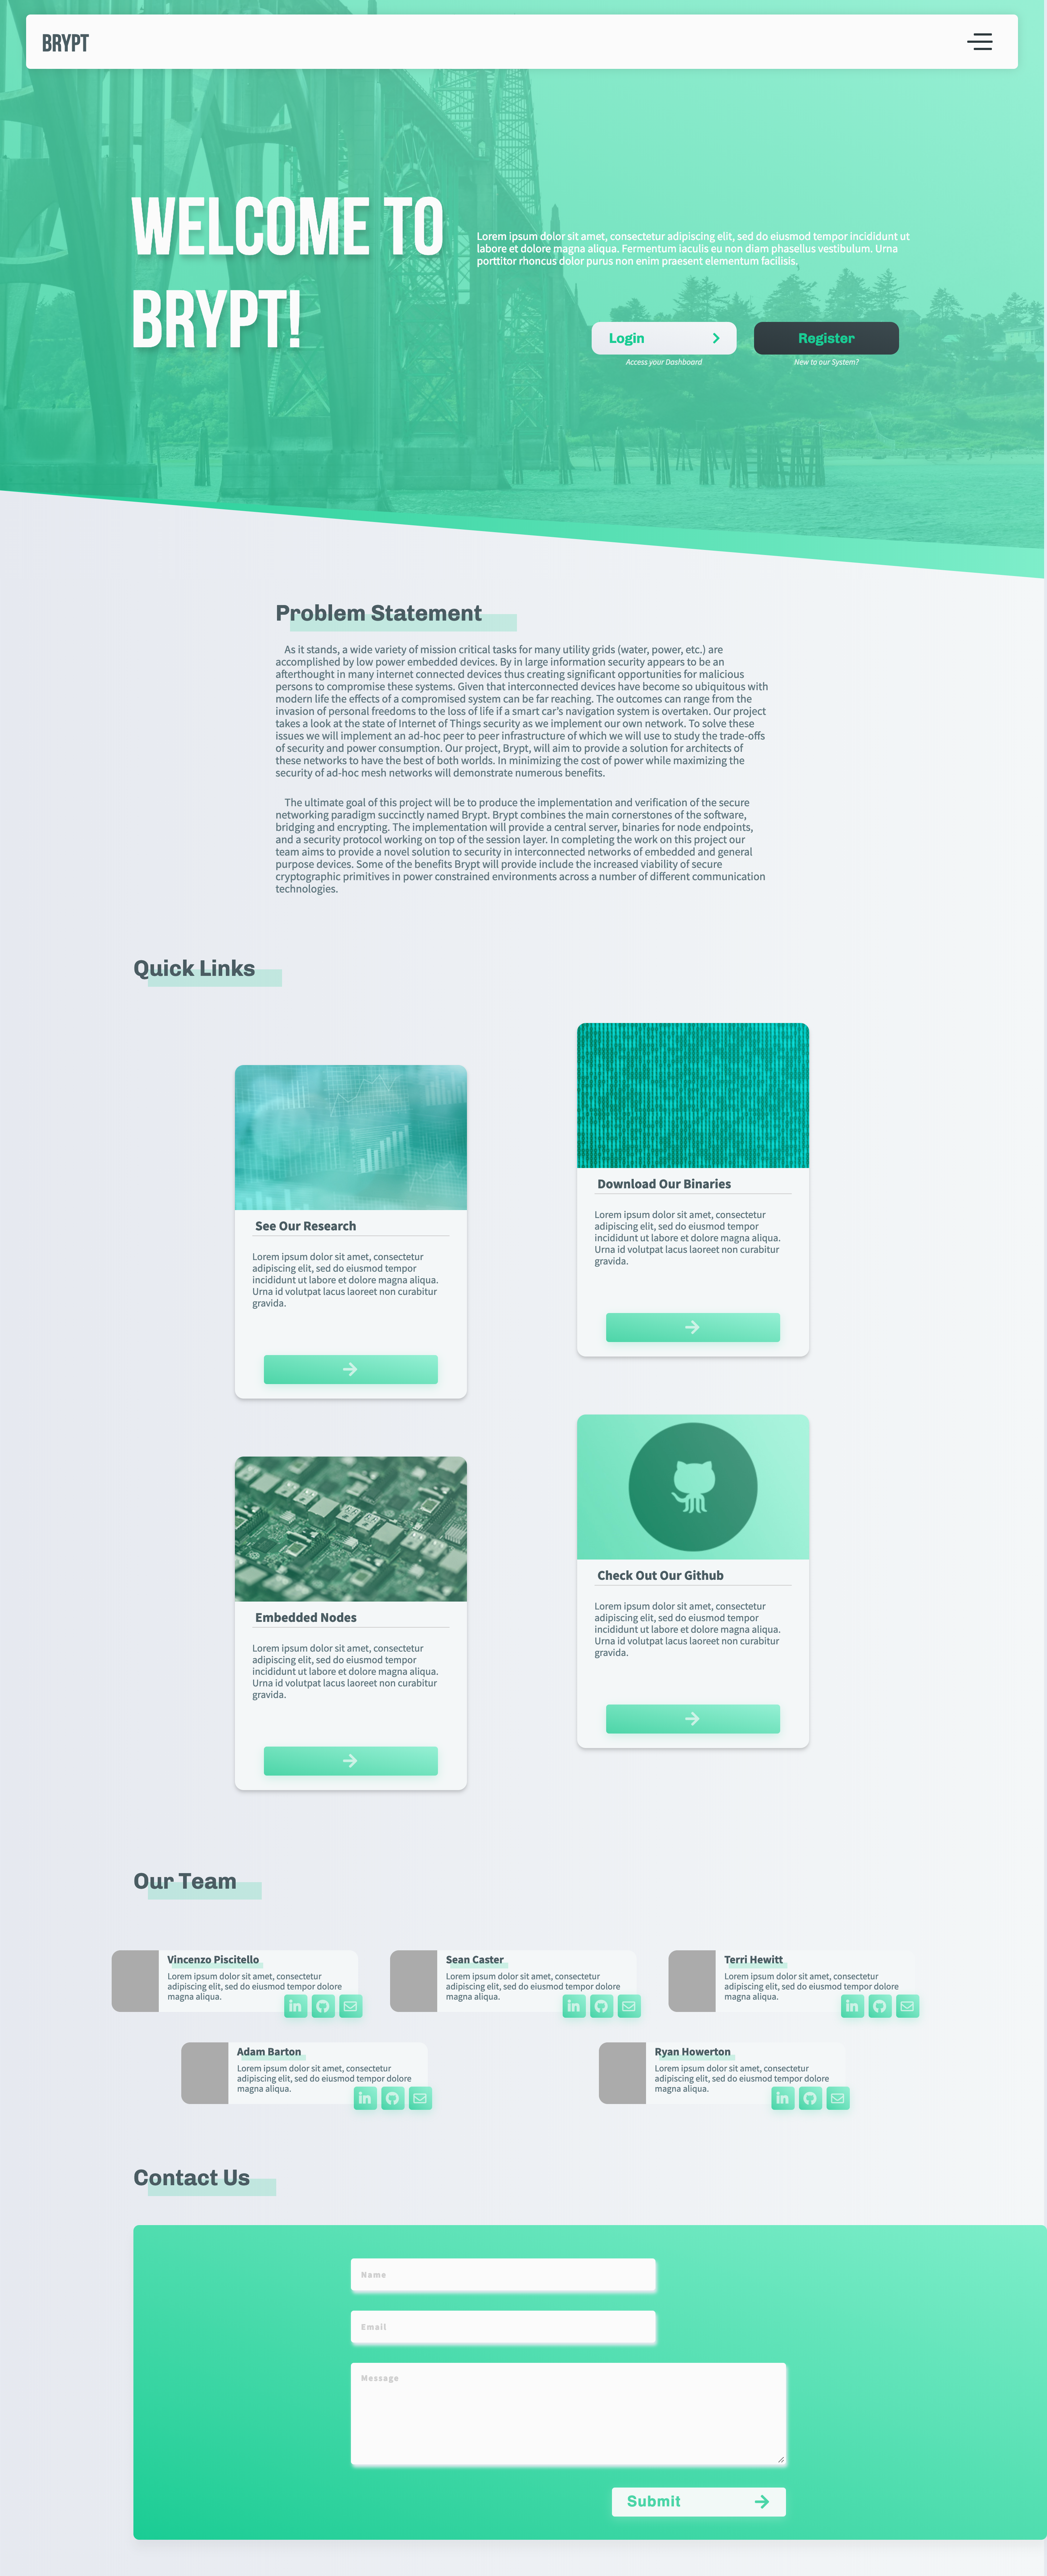
\includegraphics[scale=0.09]{brypt-home-page.png}
    \caption{Online welcome page at www.brypt.com}
\end{figure}

\section{Interesting Code Snippets}
% Message class? General diagram of MQ, msg class, polymorphism
\subsection{Desktop application supports Windows and OS X}
\lstinputlisting{./source/binding.gyp}
\subsection{AwaitObject and AwaitContainer to delay responses to requests that require input from other nodes.}
\lstinputlisting{./source/await.hpp}

%\section{Preliminary Research Results - We don't have this yet: remove?}
%\section{User Study - We don't have this: remove?}



\newpage
\section{Relevant Images}
\subsection{Brypt Architecture Diagram}
\includegraphics[width=1\linewidth]{images/working-brypt-arch.png}


\end{document}
